\chapter{Introduction}\label{sec:introduction}

This thesis is concerned with \emph{deep} neural networks, meaning
architectures consisting of many layers. Typically, the number of units
in such a model and thus the number of tunable parameters
(\(n_{weights\_per\_neuron} \times n_{neurons}\)) exceeds the number of
training examples. Training such large networks thus involves iterating
over the dataset many times which incurs a high computational cost due
to the massive number of matrix operations involved. Speeding up the
training is thus one of the primary endeavours in deep learning
research. An overview of the workings of a neural network is given in
\cref{sec:anns}.

\hypertarget{sec:anns}{%
\section{Artificial Neural Networks}\label{sec:anns}}

The artificial neural network is a class of machine learning model which can be used for regression and classification.
At it's core, neuronal models are simply conceptualized as an arrangement of units which receive inputs, compute a
weighted sum and thus produce an output activation. The ideas date back at least to Hebbian learning (a single neuron)
in the 1940s, and were developed into the Perceptron model by Rosenblatt \citep{Rosenblatt58theperceptron}. With the
introduction of the backpropagation algorithm \citep{werbos1975beyond} and increasing availability of computing power,
this began to change, but more easily trainable models like Support Vector machines eclipsed neural nets for most
applications.  Architectural advances, such as the convolutional neural networks in the late 1980's
\citep{LeCun:1989:BAH:1351079.1351090} and the advent of GPU-accelerated neural network implementations (pioneered in
\cite{Ciresan11flexible}) -- as well as subsequently, gpu-accelerated linear algebra libraries with automatic
differentiation -- finally made neural networks the cornerstone for many AI applications today.

A neural network consist of at least one input layer, \(0-n\)
intermediate layers and at least one output layer. Data is processed in
numerical form by multiplying it with the input layer's weights, mapping
each product with the input layer's activation function and then
propagating the resulting activations through subsequent layers in the
same fashion. \Cref{fig:neuralnet} gives a graphical representation of a
multi-layer feedforward network.

\begin{figure}
    \hypertarget{fig:neuralnet}{%
        \centering
        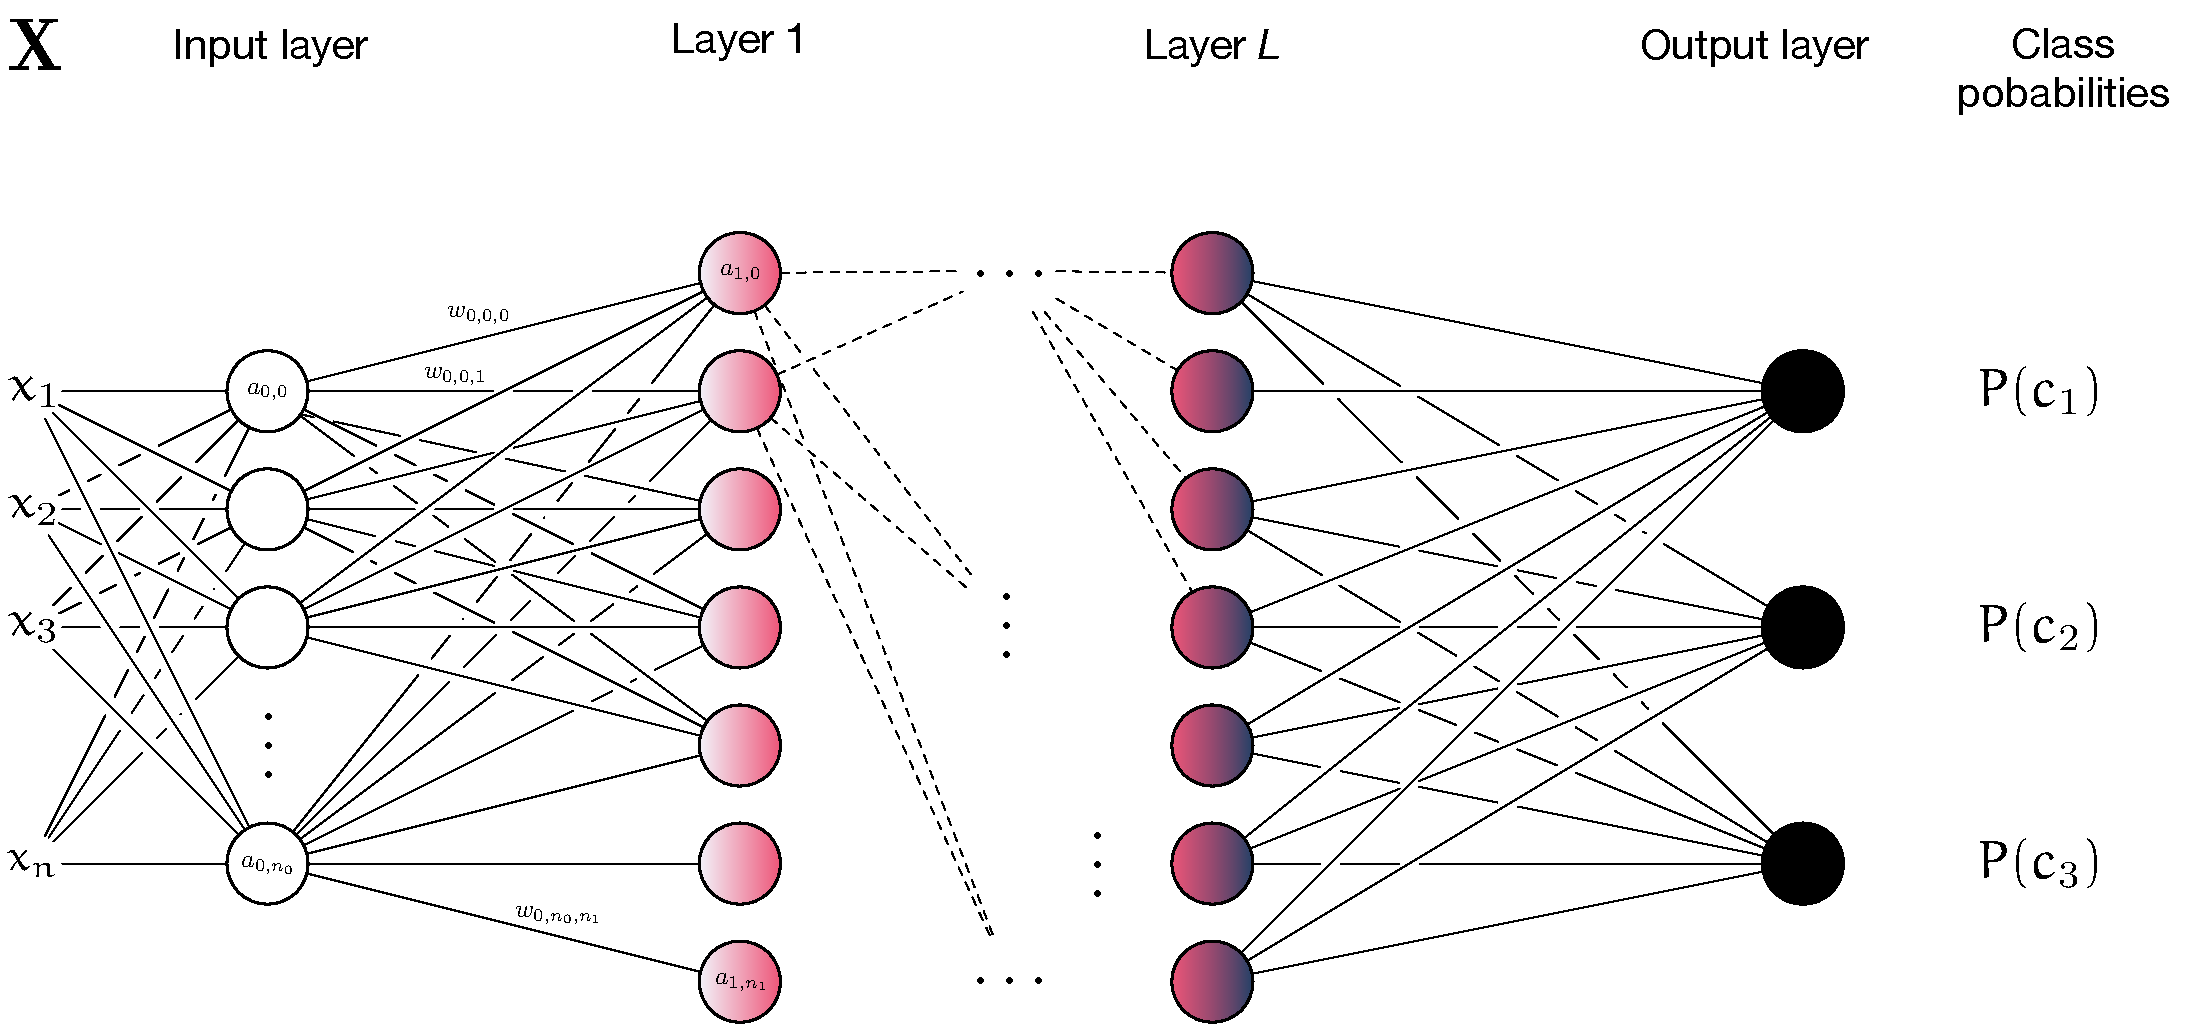
\includegraphics[max width=\textwidth]{gfx/diagrams/neural_network/neural_net.pdf}
        \caption[Schema of a multi-layer neural network]{Schema of a multi-layer neural network. \(\mathbf{x}_i\) are
            the input values, \(a_{l_n,i}\) the \(i\)-th activation in layer \(l_n\)
            and \(w_{l_n,i,j}\) the weight between the \(i\)-th unit in layer
        \(l_n\) and the \(j\)-th unit in layer \(l_{n+1}\)}\label{fig:neuralnet}
    }
\end{figure}

\hypertarget{sec:thesis-goals}{%
\section{Goals of this thesis}\label{sec:thesis-goals}}

The objective of this work is twofold:

\begin{enumerate}
    \item
        Create a software library that enables easy and reusable
        implementation of training metrics
    \item
        Perform experiments on common datasets to investigate whether common
        problems in neural network training can be detected by the use of
        appropriate metrics. Issues to be investigated are
        \begin{itemize}
            \item
                bad initializations
            \item
                inappropirate learning rate
            \item
                layer/model saturation
            \item
                inappropriate network architecture
            \item
                bad generalization/overfitting
        \end{itemize}
\end{enumerate}

\hypertarget{sec:motivation}{%
\section{Motivation}\label{sec:motivation}}

In contrast to classical machine learning models, training deep neural networks requires navigating a huge parameter
space. While most non-neural regression or classification algorithms only require specification of a parameter set
up-front and often no more than a few, some parameters can (and should) be varied over training time for neural
networks. Looking at the popular scikit-learn library, it can be seen that traditional methods such as SVMs, Gaussian
Processes, Decision Trees or Gradient Boosting typically require less than 10 algorithmic parameters.
\footnote{A look through \href{http://scikit-learn.org/stable/supervised_learning.html\#supervised-learning}{scikit-learn}s
selection of regressors and classifiers shows most classes require between 5 and 10 parameters. \citep{scikit-learn}}

In neural networks the parameter space can have arbitrarily many dimensions when factoring in the fact that some
parameters can change over time, such as

\begin{itemize}
    \item
        learning rate (can be annealed)
    \item
        batch size\footnote{It is not usual to change the batch size during
            training, but it can have an effect similar annealing the learning
        rate (see \cite{DBLP:journals/corr/abs-1711-00489})}
        \item
            trainability of layers
    \end{itemize}

    Other parameters that need to be set initially are

    \begin{itemize}
        \item
            Network architecture (how many layers, how many units per layer)
        \item
            nonlinearity function
        \item
            type of loss
        \item
            optimization algorithm
        \item
            initial learning rate
        \item
            momentum
        \item
            weight decay
    \end{itemize}

    This makes finding an optimal training regimen very hard, particularly
    since training deep neural networks for realistic problems can take much
    longer than traditional methods, meaning cross-validating different
    models can be prohibitively expensive. It is therefore desirable to
    notice dead ends early during training, or be able to tweak parameters
    in such a way as to maximize convergence speed.

    This thesis work is motivated by the scarcity of useful tools to debug
    and monitor deep learning training. Without years of training and a lot
    of mathematical intuition and expertise, it is often very hard to figure
    out why a network isn't learning or how to ensure timely convergence.
    And even with this expertise, visualizations or metrics need to be
    implemented over and over again because common tools do not abstract
    from the concrete model architecture.

    There exist a some of monitoring tools (see \cref{sec:existing-apps}),
    but they are mostly low-level tools which provide visualization
    primitives (drawing and interacting with graphs). They may enable
    visualization of certain network metrics on top of the primitives, but
    There is no native support for a concept such as \emph{Maximum singular
    value of the weight matrix} which can be simply applied automatically to
    all layers.

    In contrast, the library developed in this work is geared towards
    modularizing introspection metrics in such a way that they are usable
    for any kind of model, without modifications to the model code. The
    secondary purpose of the library is the enablement to quickly iterate on
    hypothesized metrics extracted from the training in order to diagnose
    problems such as those outlined in \cref{sec:thesis-goals}

    As such, the library shall not only be useful to end users who will make
    use of established metrics and thus save time in their model training,
    but also to researchers and the author of this thesis in for evaluating
    hypotheses about training metrics.

    \hypertarget{sec:existing-apps}{%
    \section{Existing Applications}\label{sec:existing-apps}}

    \hypertarget{tensorboard}{%
    \subsection*{TensorBoard}\label{tensorboard}}

    TensorBoard is a visulization toolkit originally developed for the TensorFlow \citep{tensorflow2015-whitepaper} deep
    learning framework. It is composed of a Python library for exporting data from the training process and a web server
    which reads the serialized data and displays it in the browser. The server can be used independently from
    TensorFlow, provided the data is serialized in the appropriate format. This enables, e.g., a PyTorch port, termed
    TensorBoardX.

    For exporting data during training, the developer adds operations to the
    graph which write scalars, histograms, audio, or other data
    asynchronously to disk. This data can then be displayed in approximately
    real-time in the web browser. Besides scalar-valued functions, which
    could be e.g.~the loss curve or accuracy measure, TensorBoard supports
    histograms, audio, and embedding data natively. However, concrete
    instances of these classes of training artifact must be defined by the
    user and can only be reused if the developer creates a separate library
    for the computations involved.

    New kinds of visualizations can be added with plugins, which require not
    only writing the Python code exporting the data and for serving it from
    the web server, but also JavaScript for actually displaying it (the
    Polymer library is used for this\footnote{\url{https://www.polymer-project.org/}}).

    An attempt to abstract over the the programming language for talking to
    the server is \href{https://github.com/torrvision/crayon}{Crayon} which
    so far supports Python and Lua.

    \hypertarget{visdom}{%
    \subsection*{Visdom}\label{visdom}}

    Visdom by Facebook Research fulfills more or less the same purpose as
    TensorBoard, but supports Numpy and Lua Torch. In contrast to
    TensorBoard, Visdom includes more features for organizing the display of
    many visualizations at once. Still, the framework is mostly geared
    towards improving workflows for data scientists, and is not concerned
    with providing useful metrics out-of-the-box.

    \hypertarget{others}{%
    \subsection*{Others}\label{others}}

    There are other tools such as
    \href{http://yosinski.com/deepvis}{DeepVis} for offline introspection,
    which offer insights into the training after the fact, but do not help
    guiding the training process while it's running.
